\chapter{Resultados Preliminares}

\section{Mezuro: Prezento}

Como dito no capítulo anterior, o Prezento é a camada da interface web do
Mezuro. Desenvolvido em Ruby on Rails, atualmente utiliza as versões 2.3.0 do
Ruby e 4.2.4 do Rails. Versões estas que estão em constante mudança, pois os
autores têm como intuito usufruir o que há de mais recente das funcionalidades
dessa tecnologia. Esta será a principal camada trabalhada neste trabalho de
conclusão de curso, pois é
nela que há a interação com o usuário. Possivelmente será utilizado um botão que
possibilitará ao usuário ter acesso e interagir com a visualização gráfica do
resultado da análise estática na mesma página ou em outra. As Figuras
\ref{fig:exmplo_disposicao_botao_visualizacao_1} e
\ref{fig:exmplo_disposicao_botao_visualizacao_2} mostram possíveis localizações
para este botão.

% TODO: atualizar estas imagens e DESTACAR botôes

\begin{figure}[!htb]
	\centering
    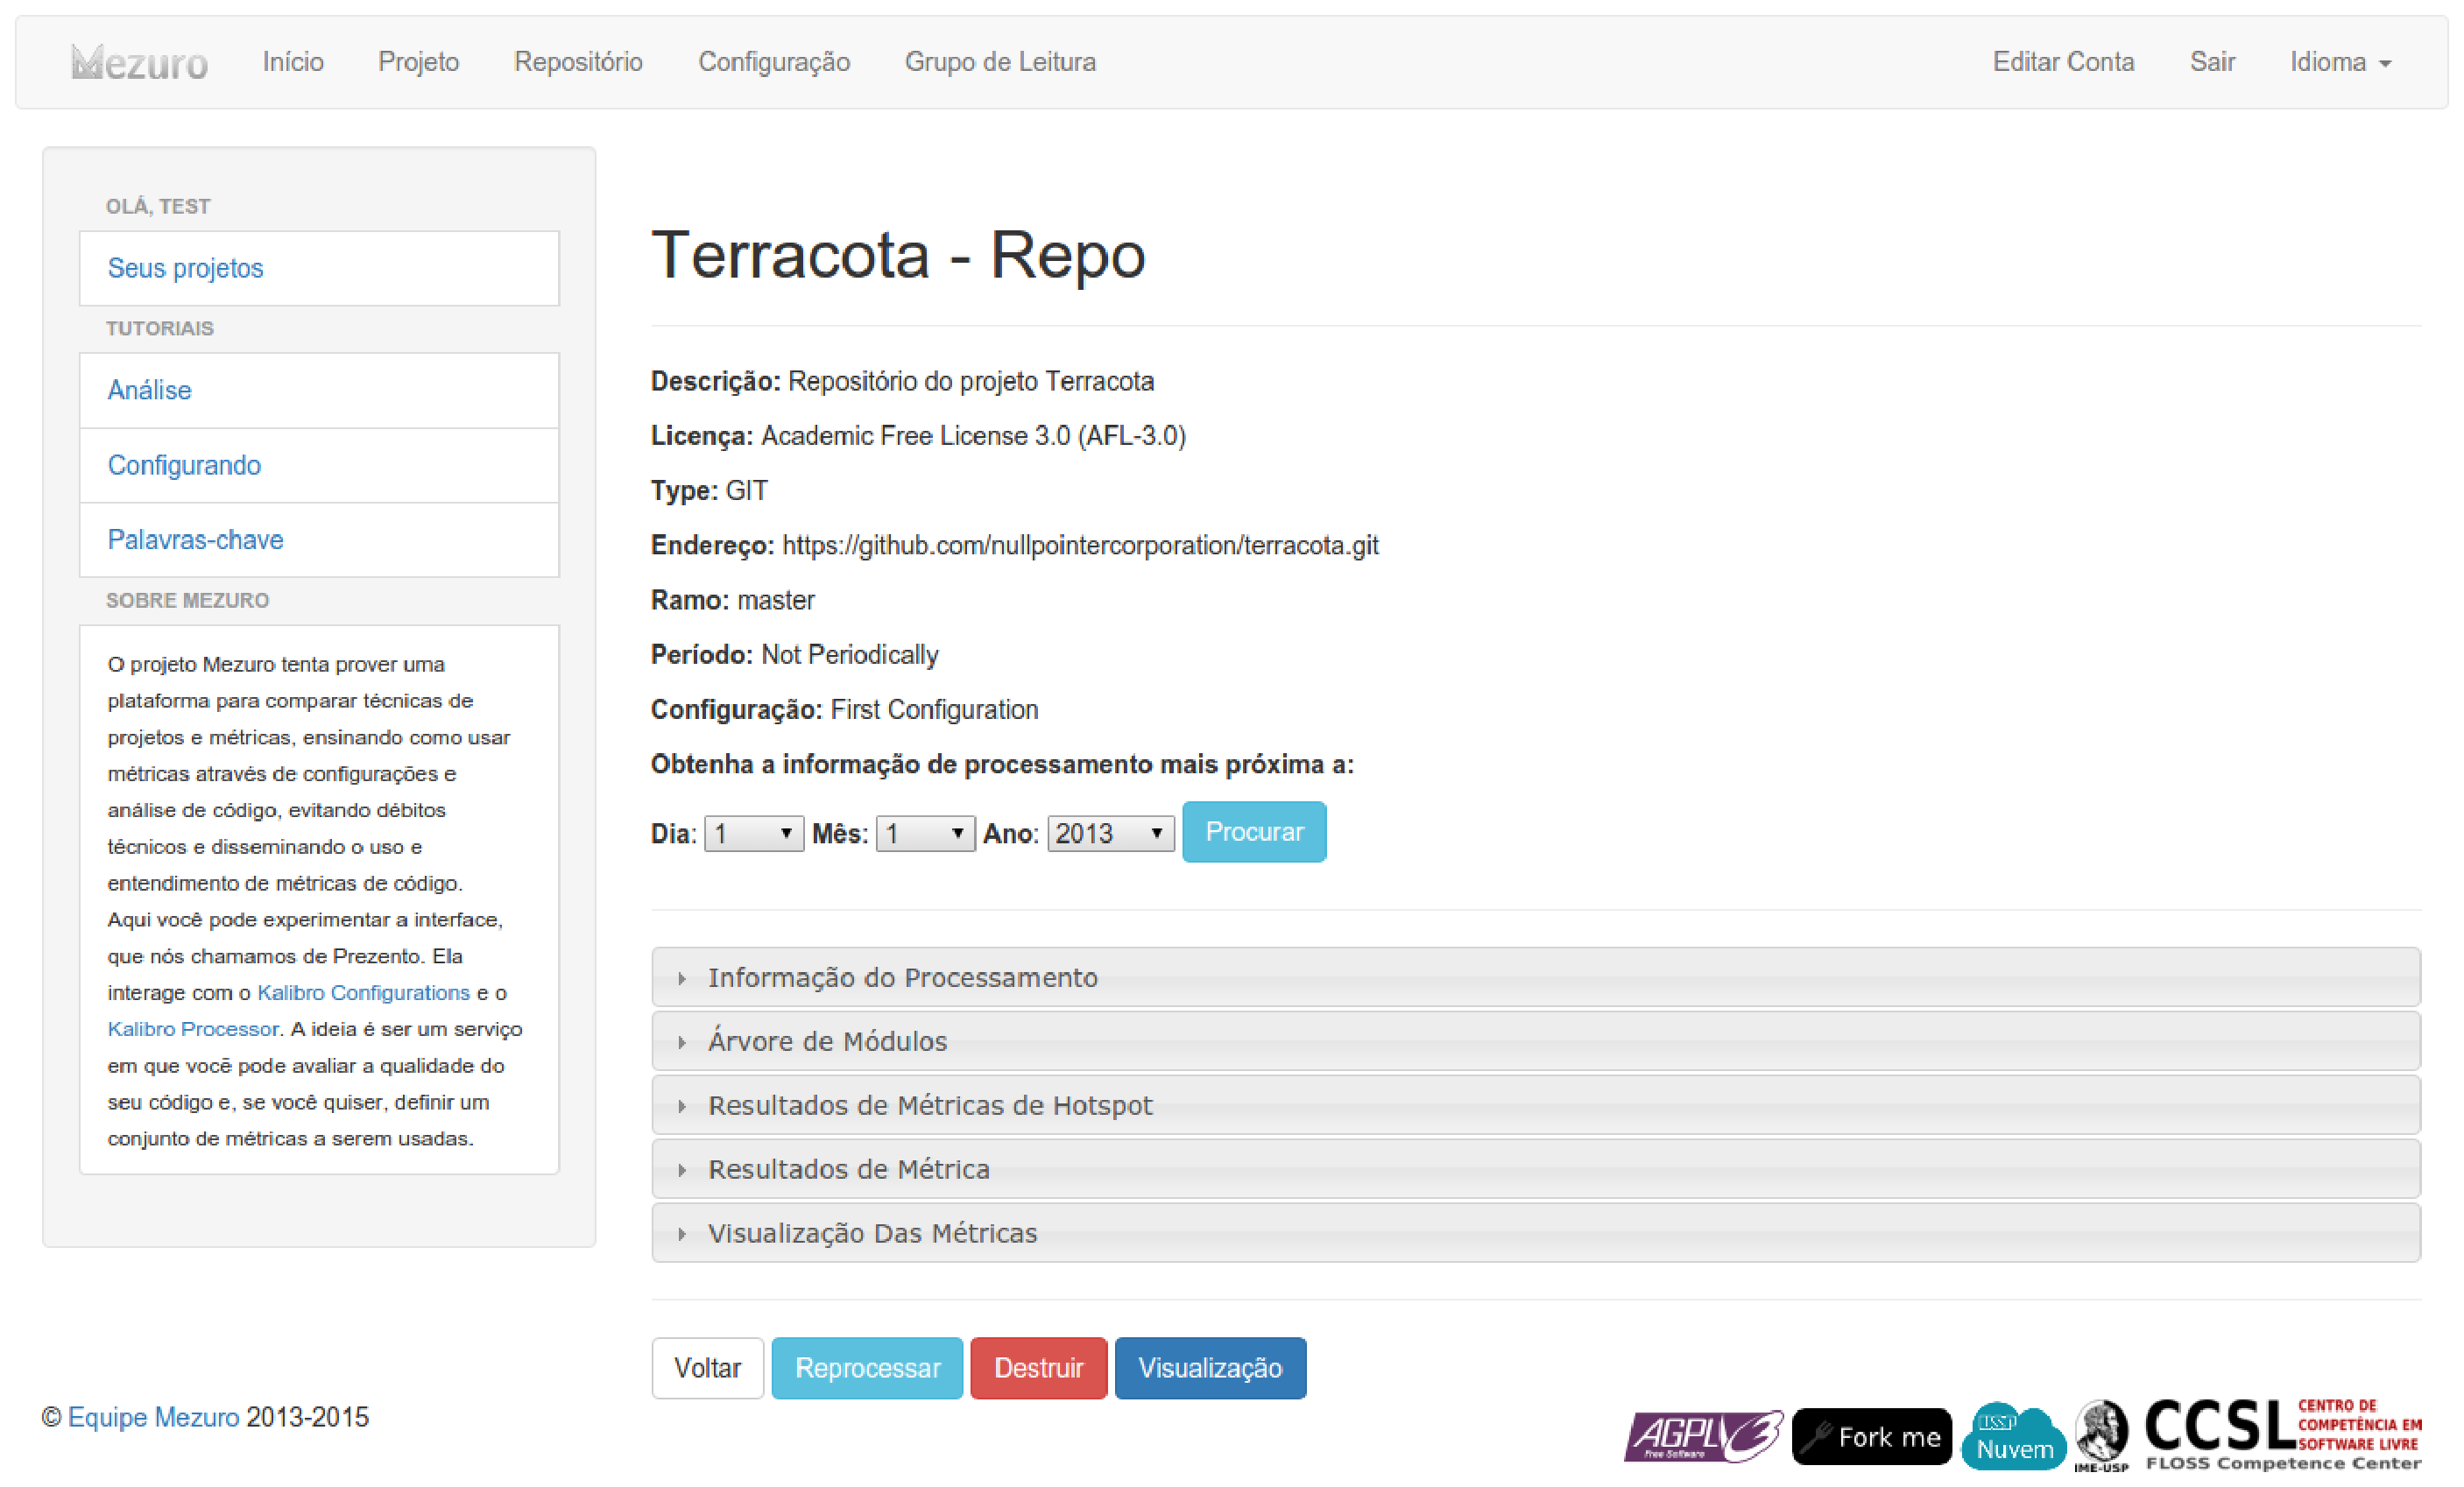
\includegraphics[keepaspectratio=true,scale=0.33]
    {figuras/exmplo_disposicao_botao_visualizacao_1.eps}
  \caption{Possíveis disposições dos botões de acesso à visualização (recolhido)}
  \label{fig:exmplo_disposicao_botao_visualizacao_1}
\end{figure}

\begin{figure}[!htb]
	\centering
    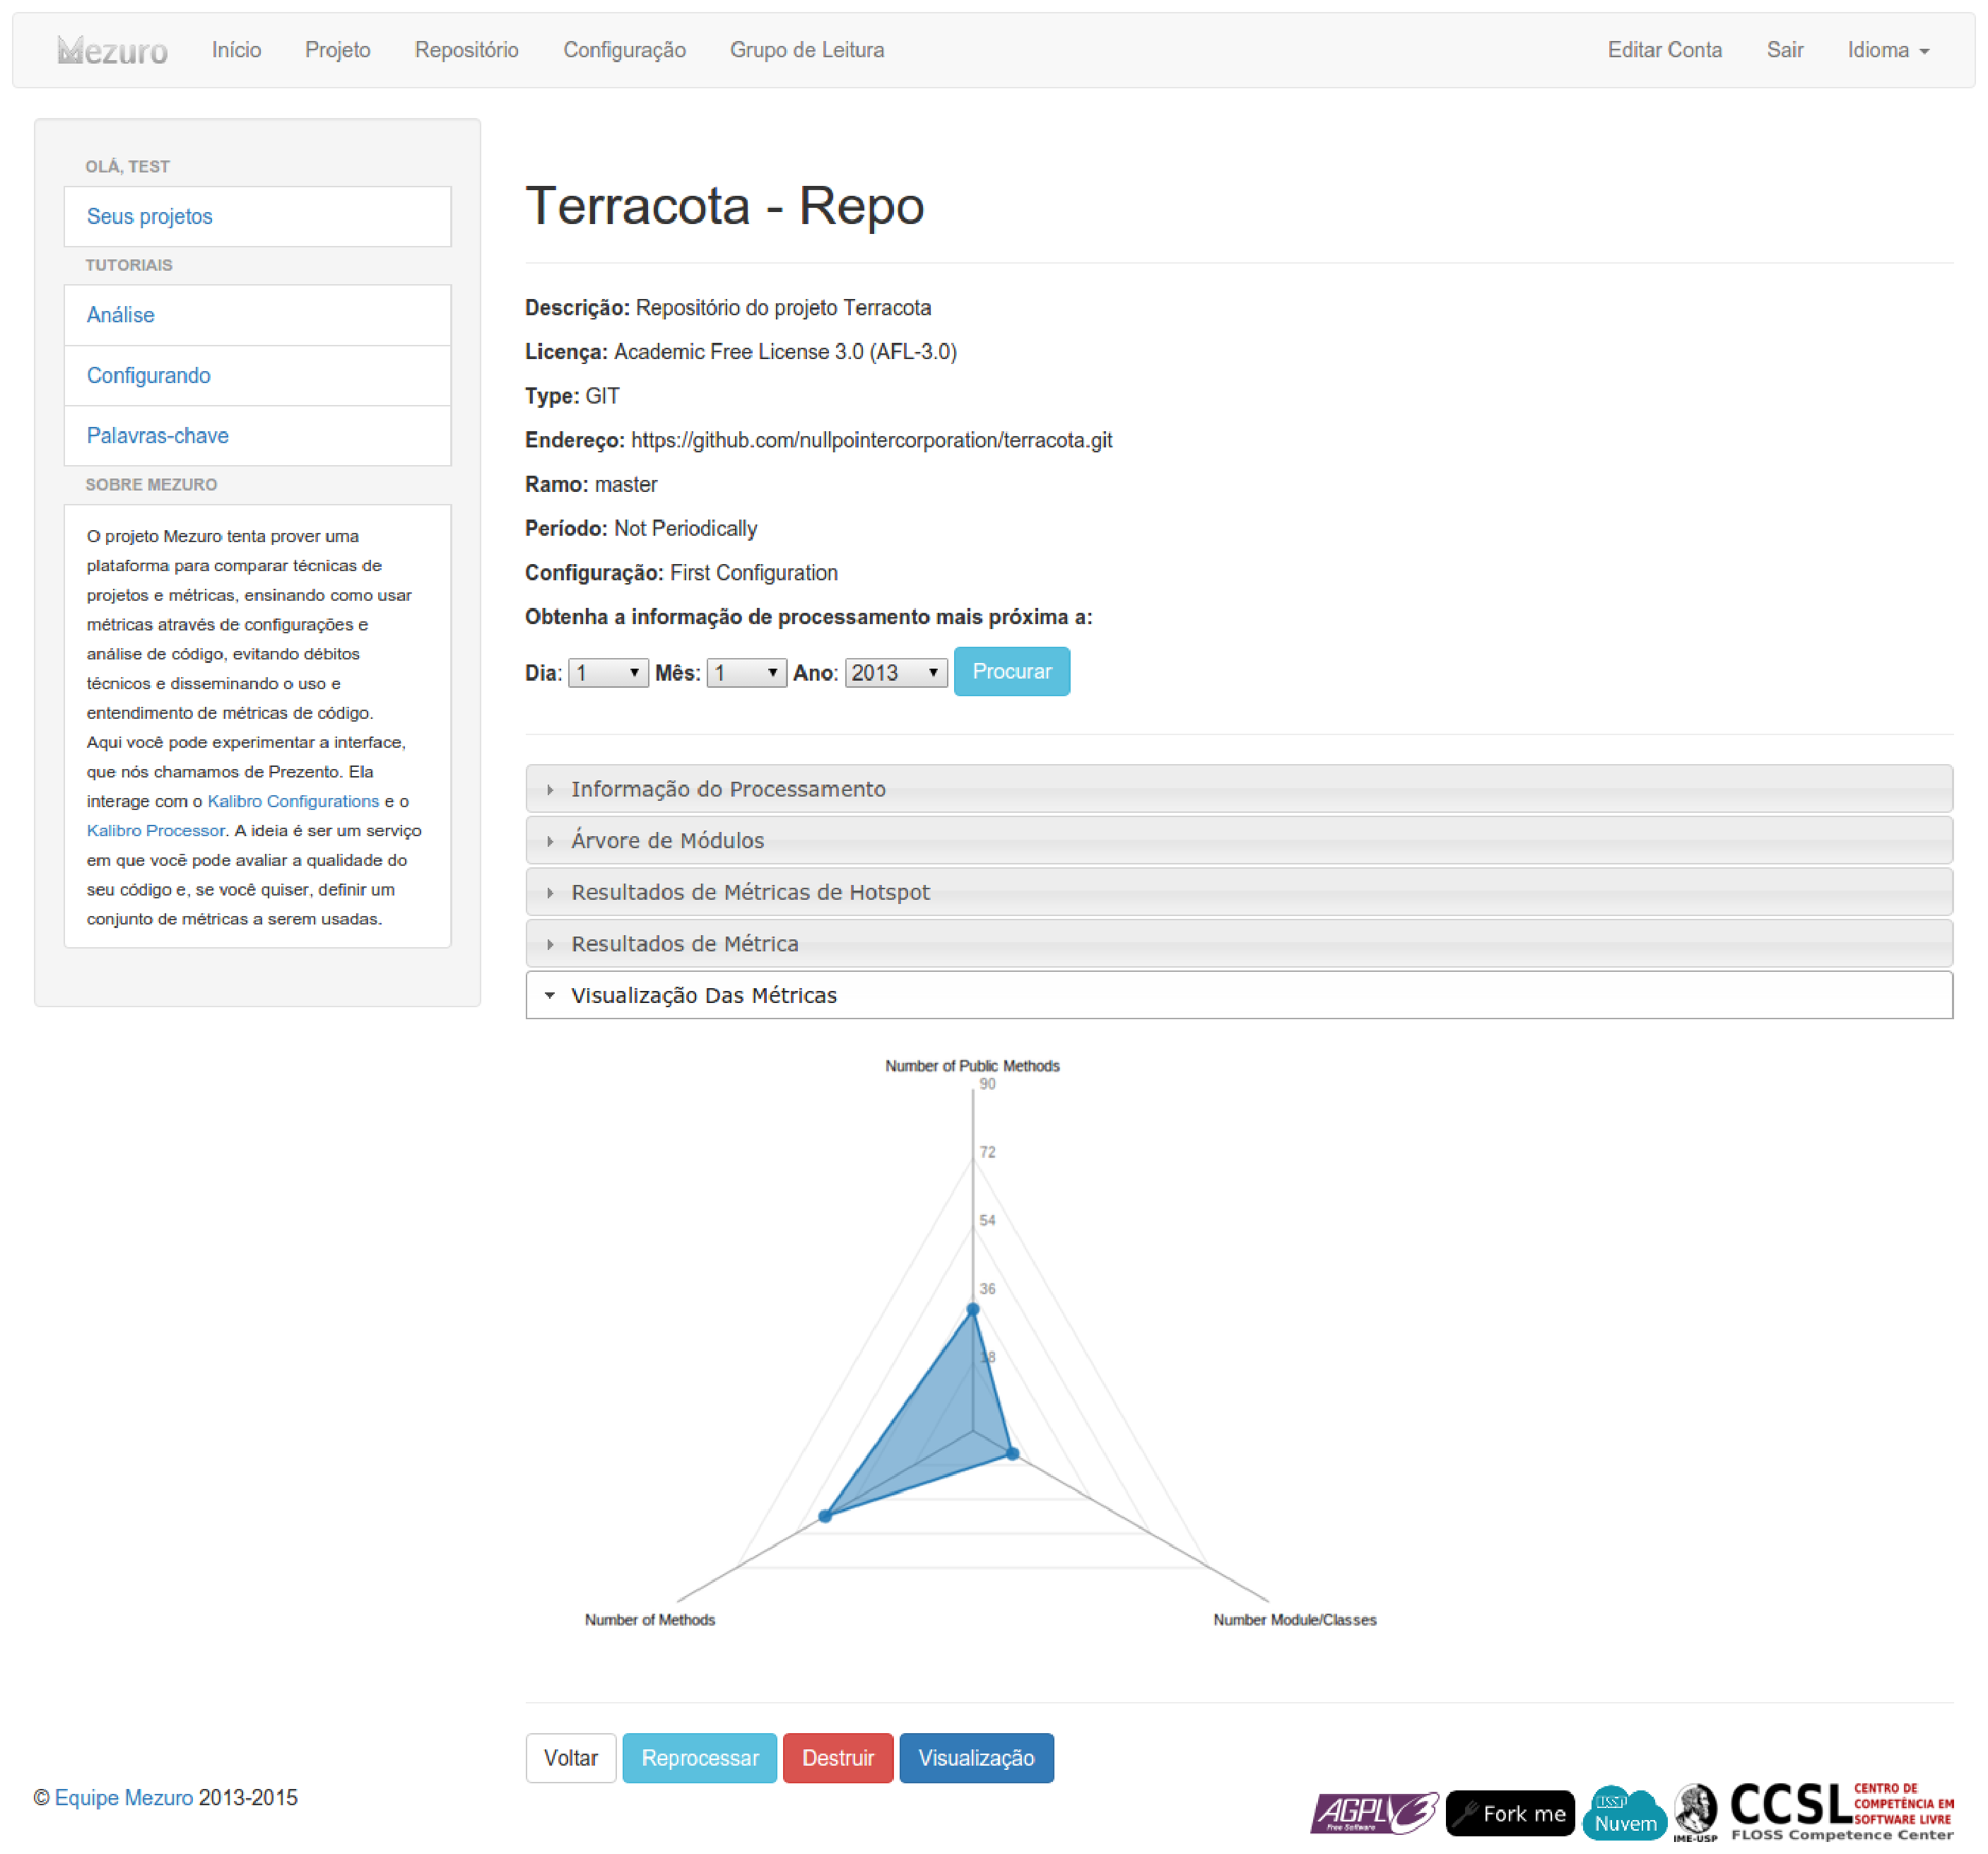
\includegraphics[keepaspectratio=true,scale=0.33]
    {figuras/exmplo_disposicao_botao_visualizacao_2.eps}
  \caption{Possíveis disposições dos botões de acesso à visualização
  (expandido) (adptado) \cite{filgueiras2014mezuro}}
  \label{fig:exmplo_disposicao_botao_visualizacao_2}
\end{figure}

\newpage

As Figuras \ref{fig:controllers_complete} e \ref{fig:models_complete} mostram os
diagramas das camadas de Controle e de Modelo do Prezento. Foram geradas com a
\textit{gem} RailRoady\footnote{\url{http://railroady.prestonlee.com/}}.

% TODO: atualizar estes diagramas

\begin{figure}[!htb]
	\centering
    \includegraphics[keepaspectratio=true,scale=0.33]
    {figuras/controllers_complete.eps}
  \caption{Diagrama da Camada de Controle}
  \label{fig:controllers_complete}
\end{figure}

\begin{figure}[!htb]
	\centering
    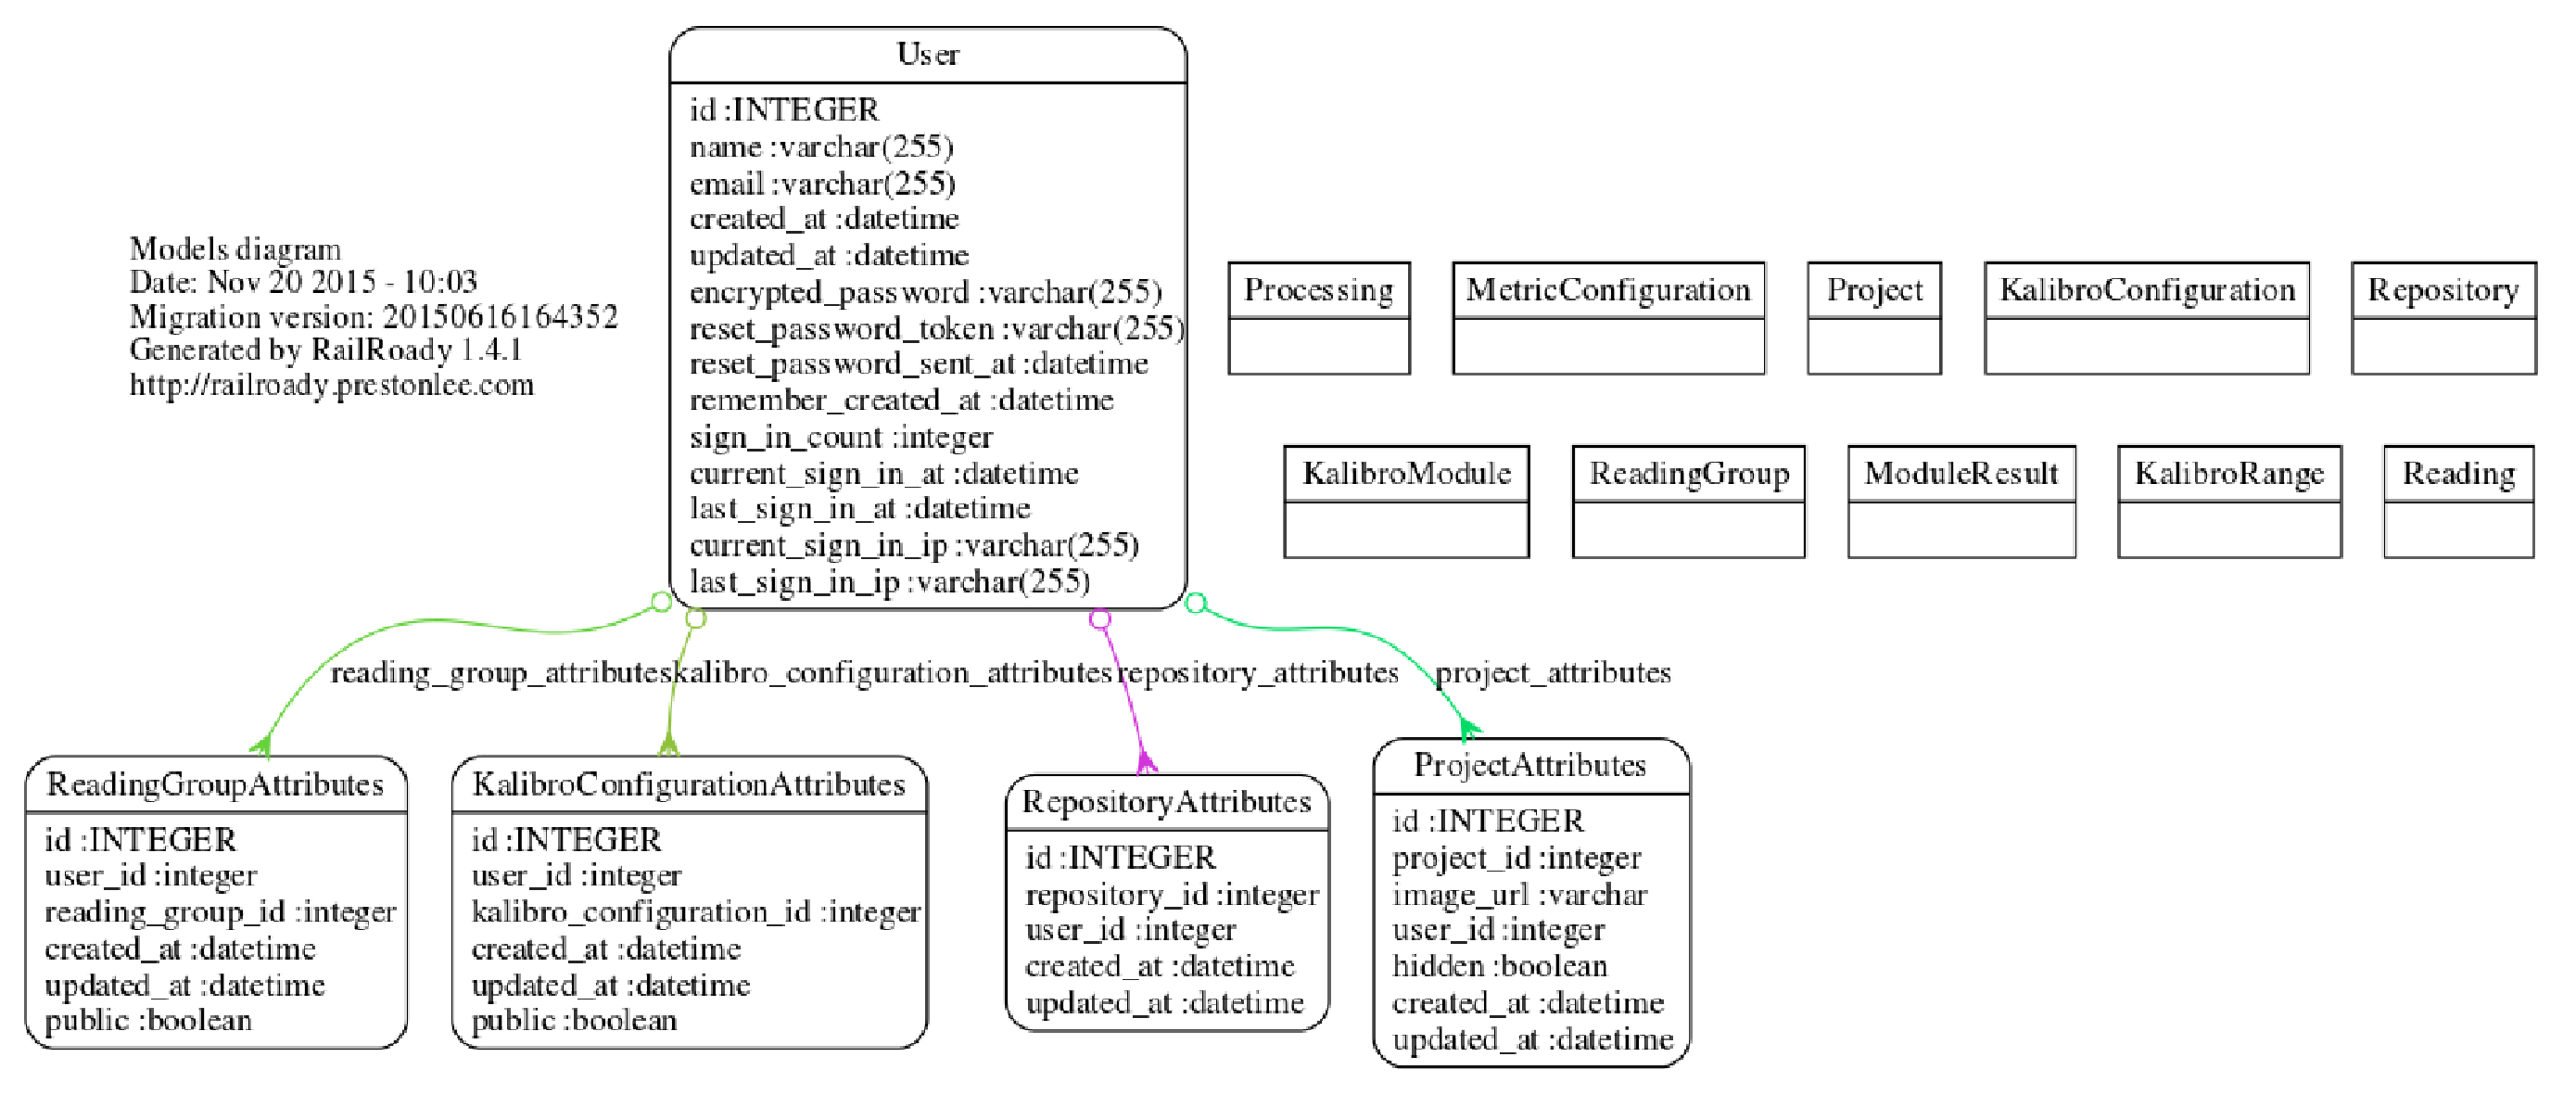
\includegraphics[keepaspectratio=true,scale=0.35]
    {figuras/models_complete_v2.eps}
  \caption{Diagrama da Camada de Modelo}
  \label{fig:models_complete}
\end{figure}

\newpage

\section{D3 - Data-Driven Documents}

D3.js (\textit{Data-Driven-Documents}) é uma biblioteca Javascript construída
inicialmente por \citeonline{bostock2011d3}, que tem como um dos seus objetivos
principais a produção de visualizações dinâmicas e interativas para a Web. Ela
faz uso de várias tecnologias vastamente utilizadas: HTML (para o conteúdo das
páginas), SVG (para descrição de gráficos vetoriais) e CSS (para estética das
páginas). A Figura \ref{fig:d3_gears} é um exemplo de como esse uso (ou
interação) é feito. Esta biblioteca permite ao programador manipular o Modelo de
Objeto de Documento (do inglês, \textit{Document Object Model} - DOM), para
modificar determinada seleção de elementos na página. Essa modificação, seja
adição ou remoção de elementos, depende dos dados de entrada e é onde a
aplicação de transformações dinâmicas é feita. Os autores idealizaram a união de
três preocupações: compatibilidade, depuração e desempenho \cite{bostock2011d3}.

\begin{figure}[!htb]
	\centering
    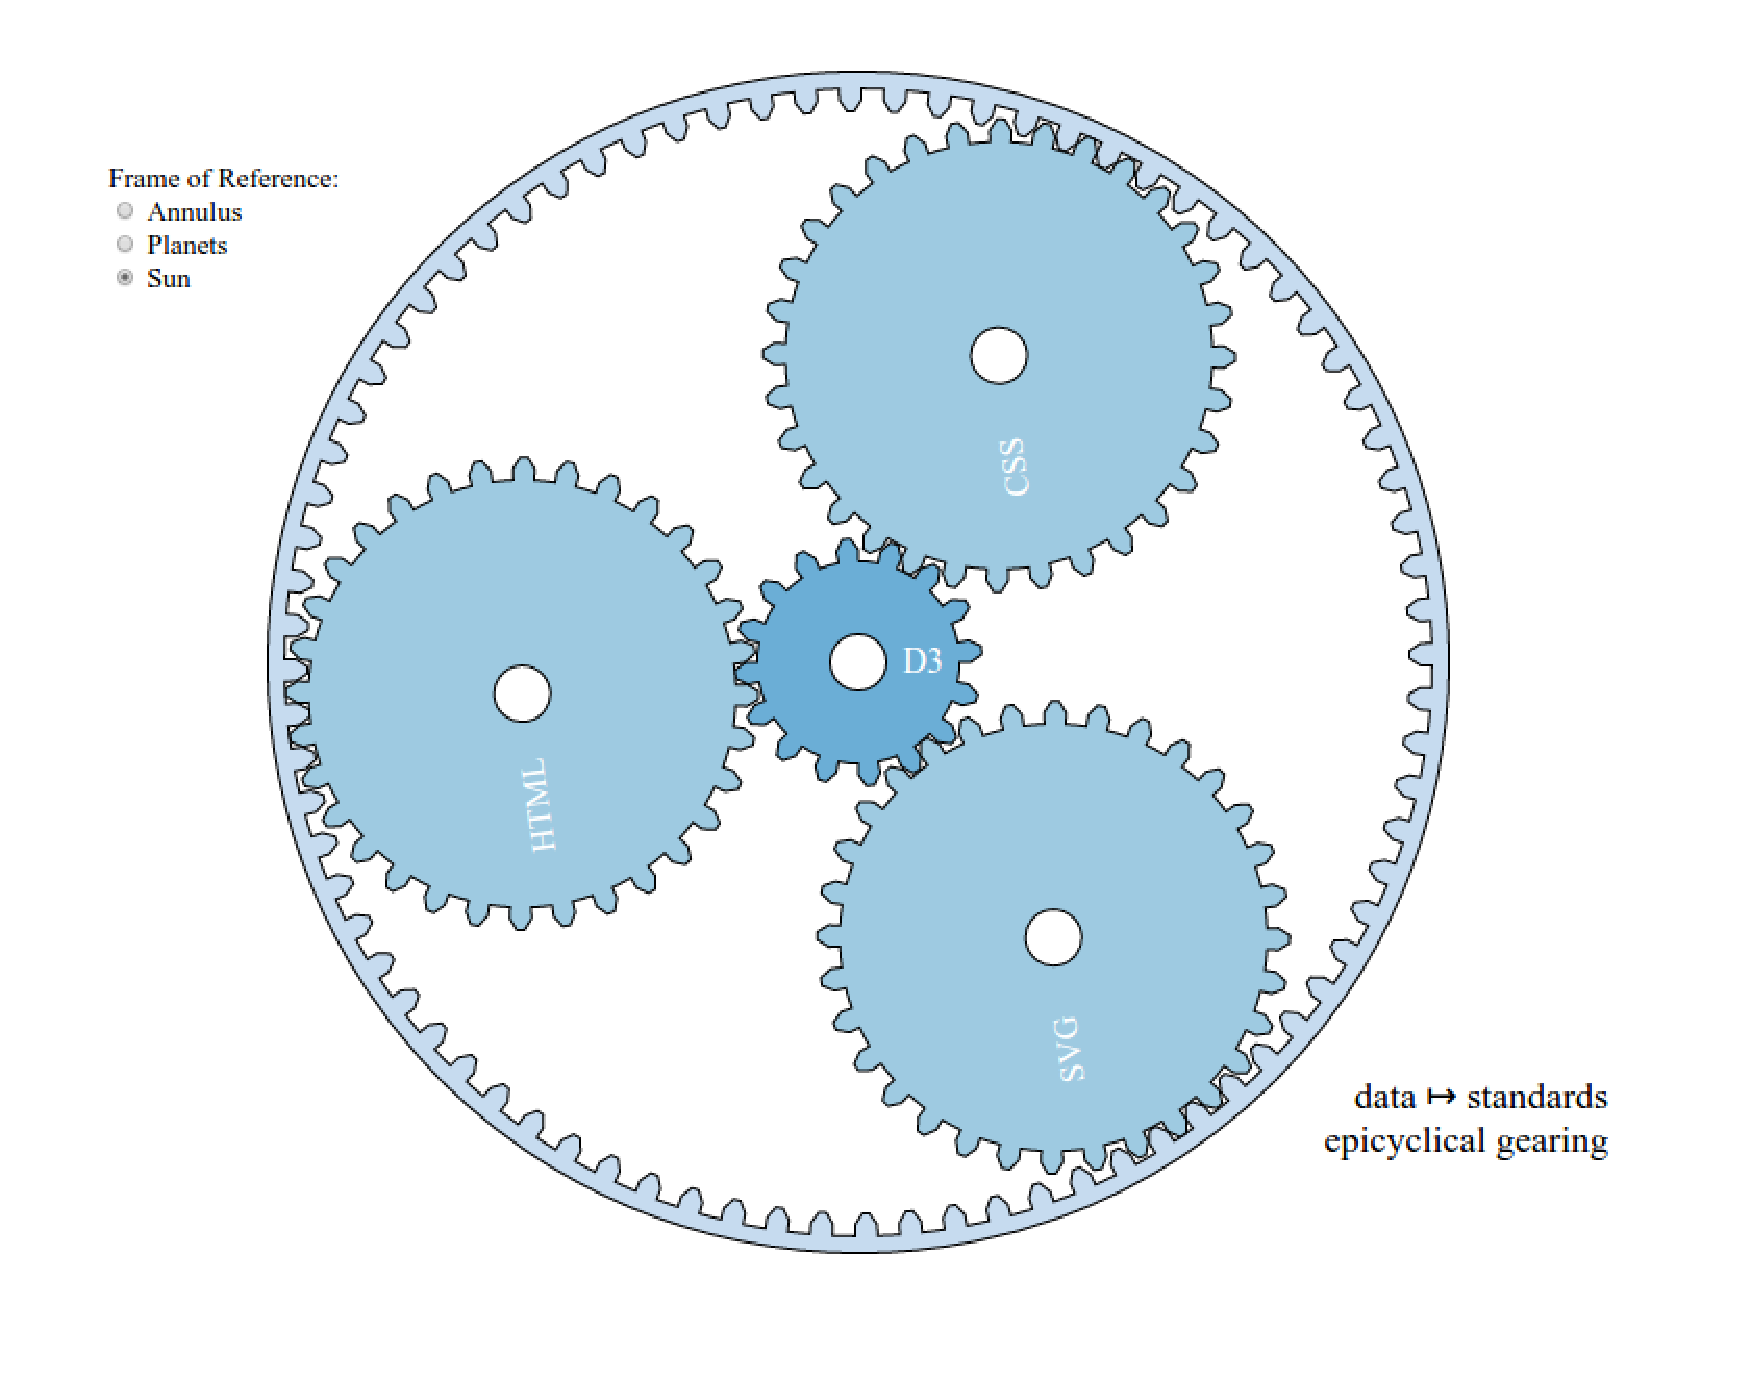
\includegraphics[keepaspectratio=true,scale=0.5]
    {figuras/d3_gears.eps}
  \caption{Exemplificação do Uso das Tecnologias pela D3.js \cite{michaeld3}}
  \label{fig:d3_gears}
\end{figure}

A biblioteca D3.js é licenciada sob a \textit{BSD licenses}, que é compatível
com a licença do Mezuro (\textit{AGPL} - \textit{Version} 3) e possui uma vasta
galeria de exemplos que podem se adaptar ao proposto neste trabalho.

\begin{figure}[!htb]
	\centering
    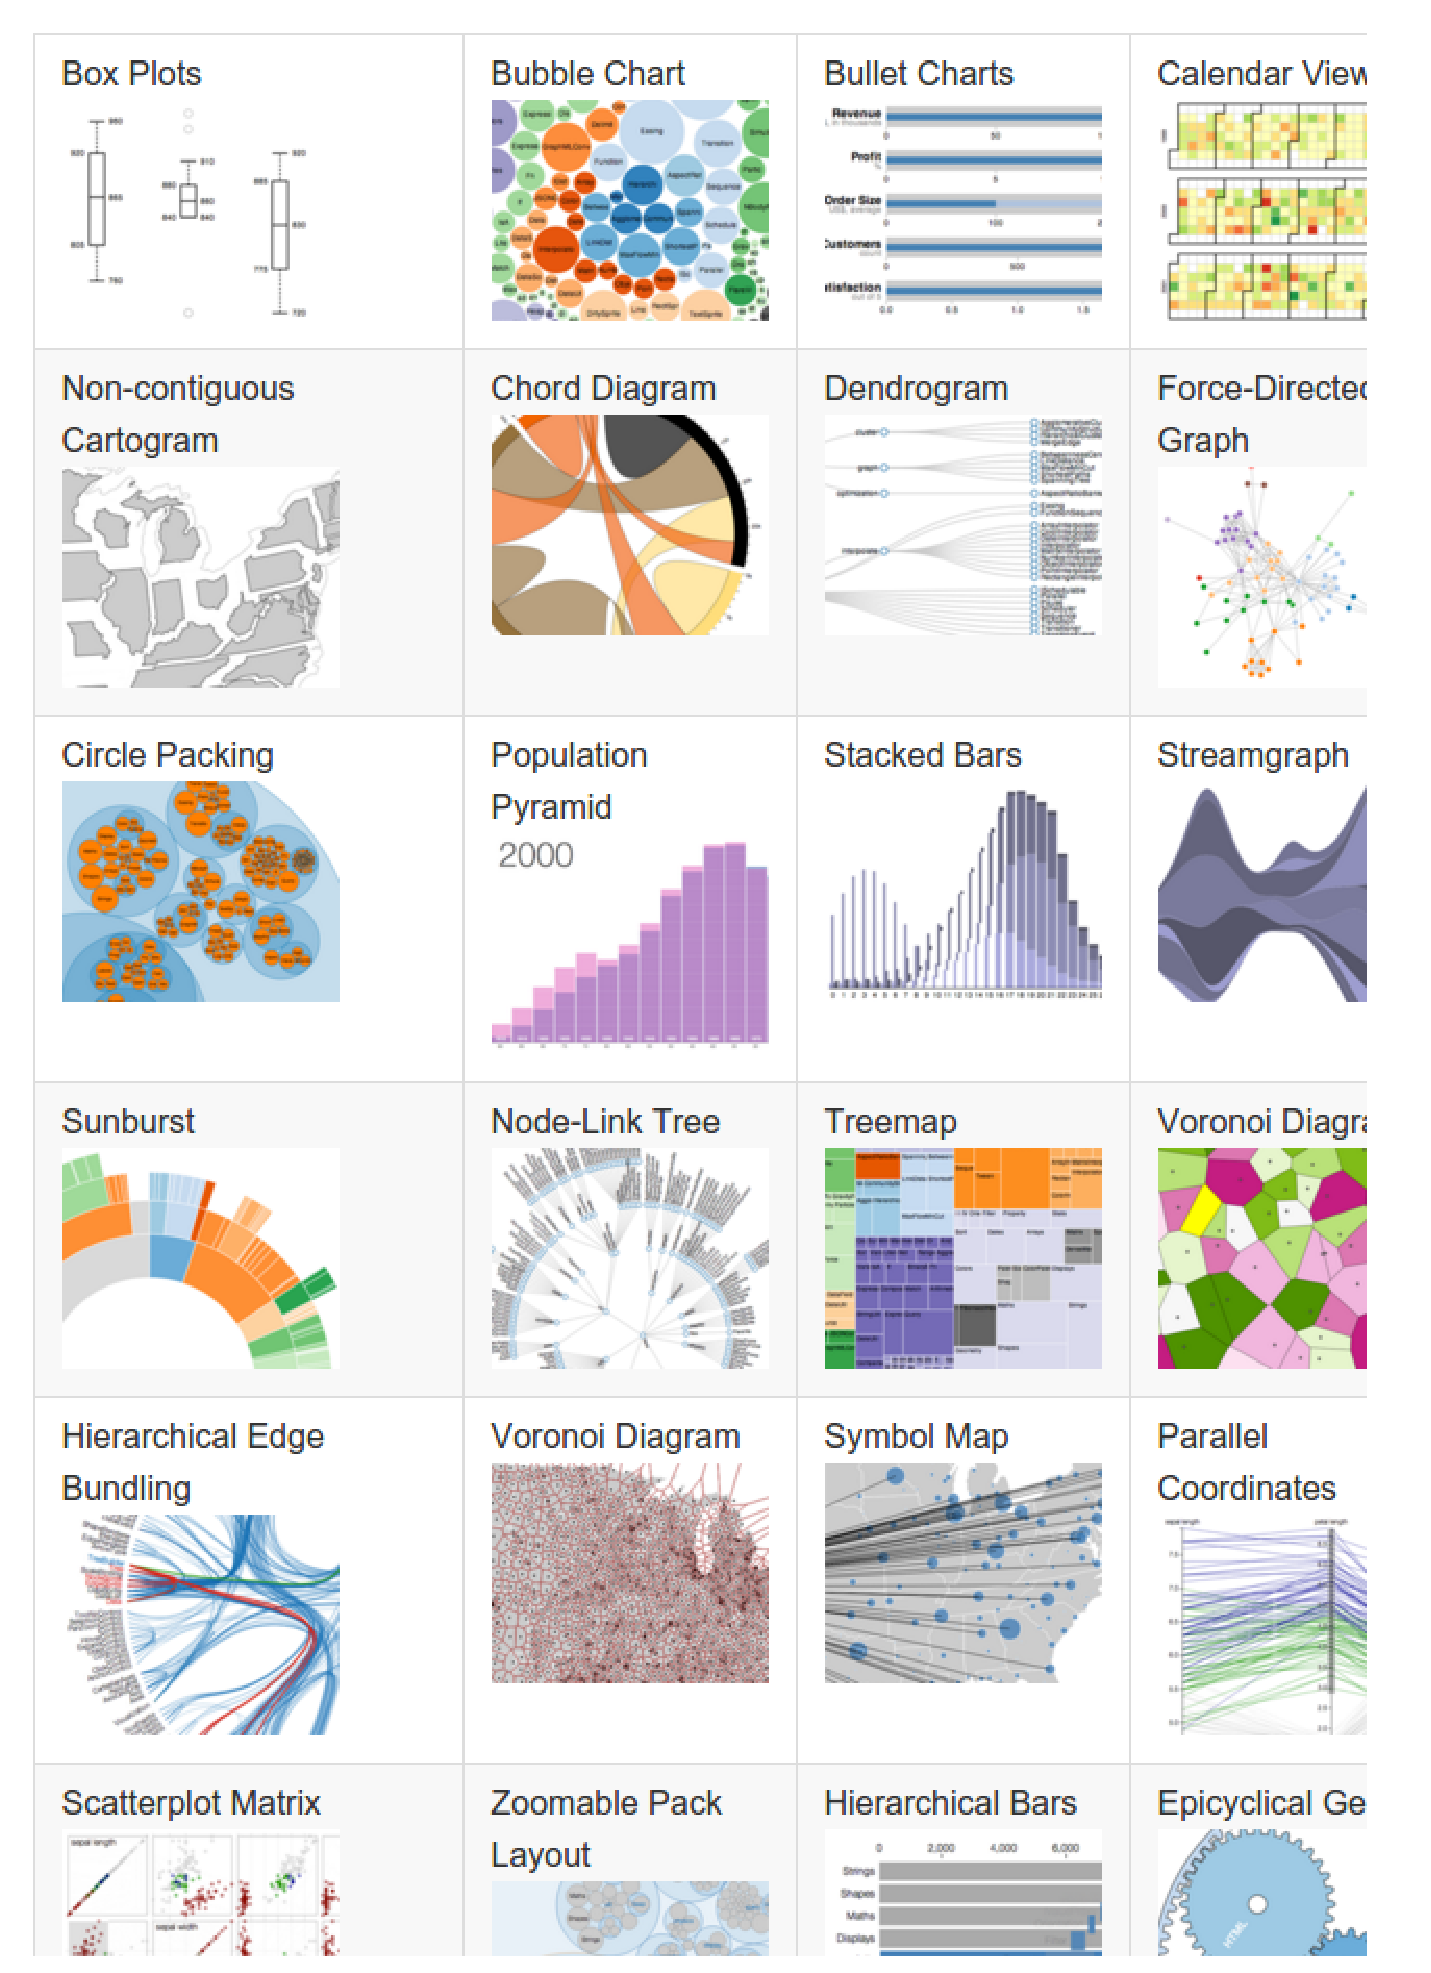
\includegraphics[keepaspectratio=true,scale=0.5]
    {figuras/d3_gallery.eps}
  \caption{Galeria de Exemplos da biblioteca D3.js \cite{galleryD3}}
  \label{fig:d3_gallery}
\end{figure}

https://github.com/mbostock/d3/wiki/Gallery

\section{Exemplo de Uso}

% TODO: escolher 3 projetos para serem alvo
% TODO: escolher quais métricas

Como prova de conceito, foi realizado a adaptação de três visualizações dos
exemplos disponíveis na galearia da biblioteca D3. A primeira, feita por Thomas
Preusse, tem como título \textit{Radar Chart}
\footnote{\url{http://bl.ocks.org/tpreusse/2bc99d74a461b8c0acb1}}. Nesta
primeira adaptação, os valores de três métricas são gerados aleatoriamente. As
métricas foram escolhidas apenas para fins de ilustração. São elas: número de
métodos, número de métodos públicos e total de módulos.

Para a segunda e terceira adaptações foram coletadas métricas do projeto da
\textit{engine} para jogos do professor Edson Alves da Costa Júnior, levando-se
em consideração apenas três classes (Animation, MouseButtonEvent e Level). As
métricas são da configuração inicial do Mezuro para projetos Java/C/C++. As
métricas são:

% TODO: Adicionar estas siglas no arquivo de abreviaturas

\begin{itemize}
  \item \textbf{ACC} (\textit{Afferent Connections per Class} - Conexões
	aferentes de uma classe)
  \item \textbf{ACCM} (\textit{Average Cyclomatic Complexity per Method} -
	Média da Complexidade Ciclomática por método)
  \item \textbf{AMLOC} (\textit{Average Method LOC} - Média do número de linhas
	de código por método)
  \item \textbf{ANPM} (\textit{Average Number of Parameters per Method} - Média
	do número de linhas de código por método)
  \item \textbf{DIT} (\textit{Depth of Inheritance Tree} - Profundidade da
	árvore de herança)
  \item \textbf{NOM} (\textit{Number of Methods} - Número de métodos)
  \item \textbf{NPA} (\textit{Number of Public Attributes} - Número de
	atributos públicos)
  \item \textbf{SC} (\textit{Structural Complexity} - Complexidade estrutural)
\end{itemize}

A segunda adaptação foi baseada no trabalho de Michael Bostock, \textit{Node
Link Tree, Radial Reingold – Tilford Tree}
\footnote{\url{http://bl.ocks.org/tpreusse/2bc99d74a461b8c0acb1}}. E a terceira
é adaptada de uma das visualizações criadas por Lars Kotthoff\footnote{\url{http://bl.ocks.org/larskotthoff/7022289}}.

Para a exibição destas adaptações, foi realizado a construção de uma aplicação
Rails simplificada, apenas com o carregamento de páginas estáticas e hospedada
na plataforma Heroku. Pode ser acessada através do domínio \href{https://visualizationtest.herokuapp.com/}{visualizationtest.herokuapp.com}.

Com o propósito de ser um teste de visualização de software, esta exibição foi
submetida à avaliação de estudantes e pessoas envolvidas com a Engenharia de
Software. Utilizou-se da ferramenta Google Forms para tal pesquisa. Foi exposto
o seguinte texto de introdução:


\begin{itemize}
  \item[] \textit{Olá!}
  \item[] \textit{Esse questionário tem o objetivo de me ajudar com o meu
	projeto de TCC.}
  \item[] \textit{A primeira considera três métricas básicas (número de
	métodos, número de métodos públicos e o número total de módulos) de um
	projeto qualquer.}
  \item[] \textit{A segunda e a terceira são métricas coletadas do projeto da
	engine para jogos do professor Edson Alves da Costa Junior(1) e considerando
	apenas três classes (Animation, MouseButtonEvent e Level). As métricas são da
	configuração geral para projetos JAVA/C/C++ do Mezuro(2).}
	\item[] \textit{Por favor, acesse https://visualizationtest.herokuapp.com/ e
	navegue pelos três links. Veja se achou intuitivo e fácil de utilizar. Após
	ter passadas pelas três visualizações, responda essas perguntas:}
	\item[] \textit{Referências}
	\item[] \textit{(1) https://github.com/fgagamedev/IJE}
	\item[] \textit{(2) http://mezuro.org/pt/kalibro\_configurations/1}
\end{itemize}

E as perguntas foram:

\begin{itemize}
  \item[] \textit{Qual das visualizações você considera melhor para a
	interpretação das métricas?}
		\subitem{Random Radar Chart by Thomas Preusse (adapted)}
		\subitem{Node Link Tree by Mike Bostock (adapted)}
		\subitem{Node Link With Interation by Lars Kotthoff (adapted)}
  \item[] \textit{Qual delas foi mais claro identificar os
	pontos/classes/métricas críticos e que merecem atenção?}
		\subitem{Random Radar Chart by Thomas Preusse (adapted)}
		\subitem{Node Link Tree by Mike Bostock (adapted)}
		\subitem{Node Link With Interation by Lars Kotthoff (adapted)}
  \item[] \textit{Por favor, caso tenha algum comentário, críticas e sugestões,
	utilize o campo abaixo:}
\end{itemize}

As figura \ref{fig:radar}, \ref{fig:node_link_tree} e
\ref{fig:node_link_tree_with_interaction} mostram estas adaptações disponíveis
na pequena aplicação Rails.

\begin{figure}[!htb]
	\centering
    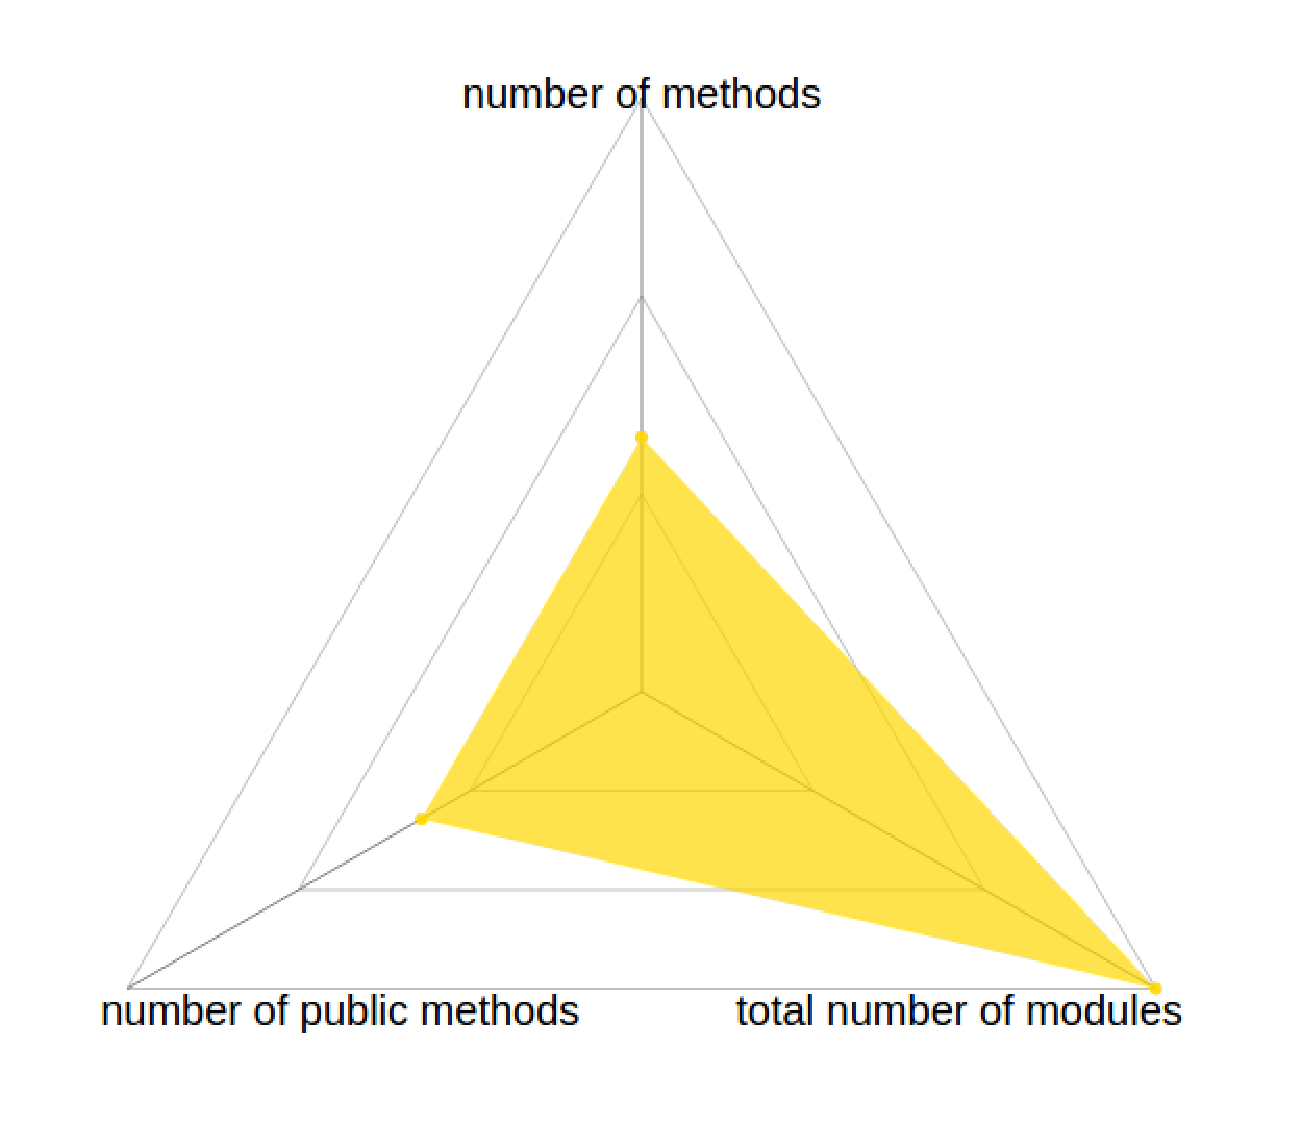
\includegraphics[keepaspectratio=true,scale=0.5]
    {figuras/radar.eps}
  \caption{Gráfico Radar por Thomas Preusse (adaptado)}
  \label{fig:radar}
\end{figure}

\begin{figure}[!htb]
	\centering
    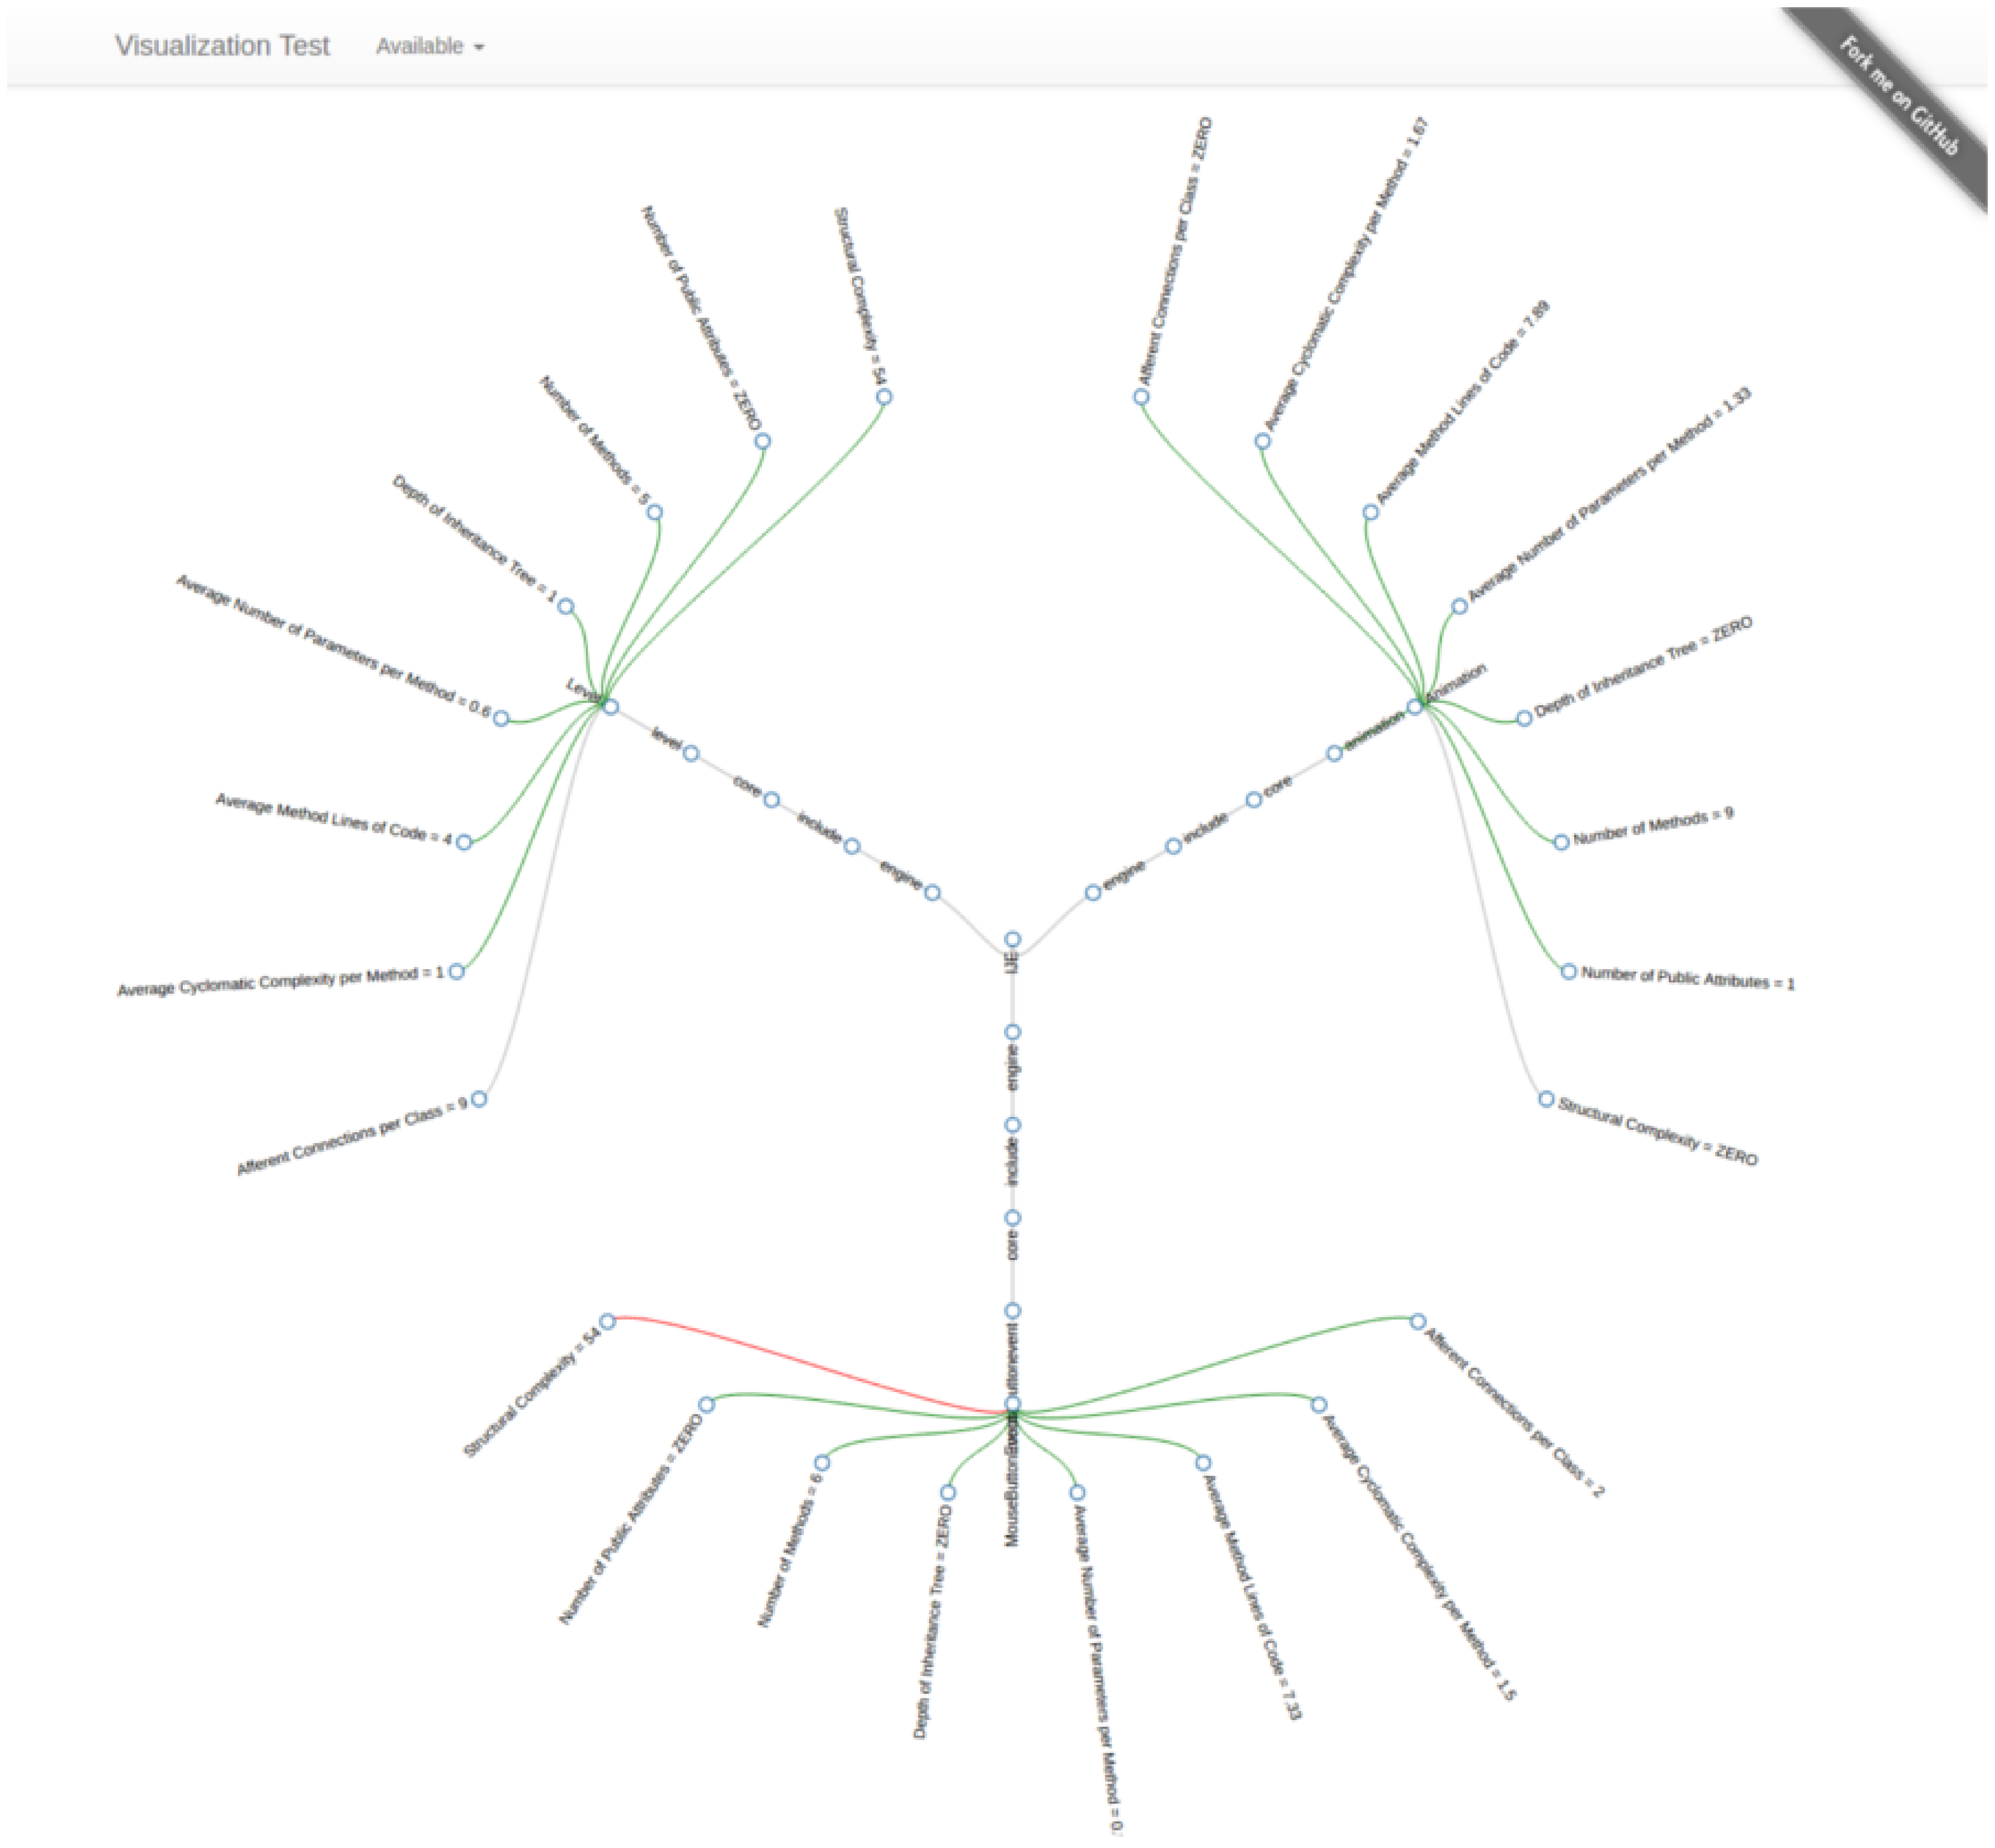
\includegraphics[keepaspectratio=true,scale=0.15]
    {figuras/node_link_tree.eps}
  \caption{Node Link Tree por Michael Bostock (adaptado)}
  \label{fig:node_link_tree}
\end{figure}

\begin{figure}[!htb]
	\centering
    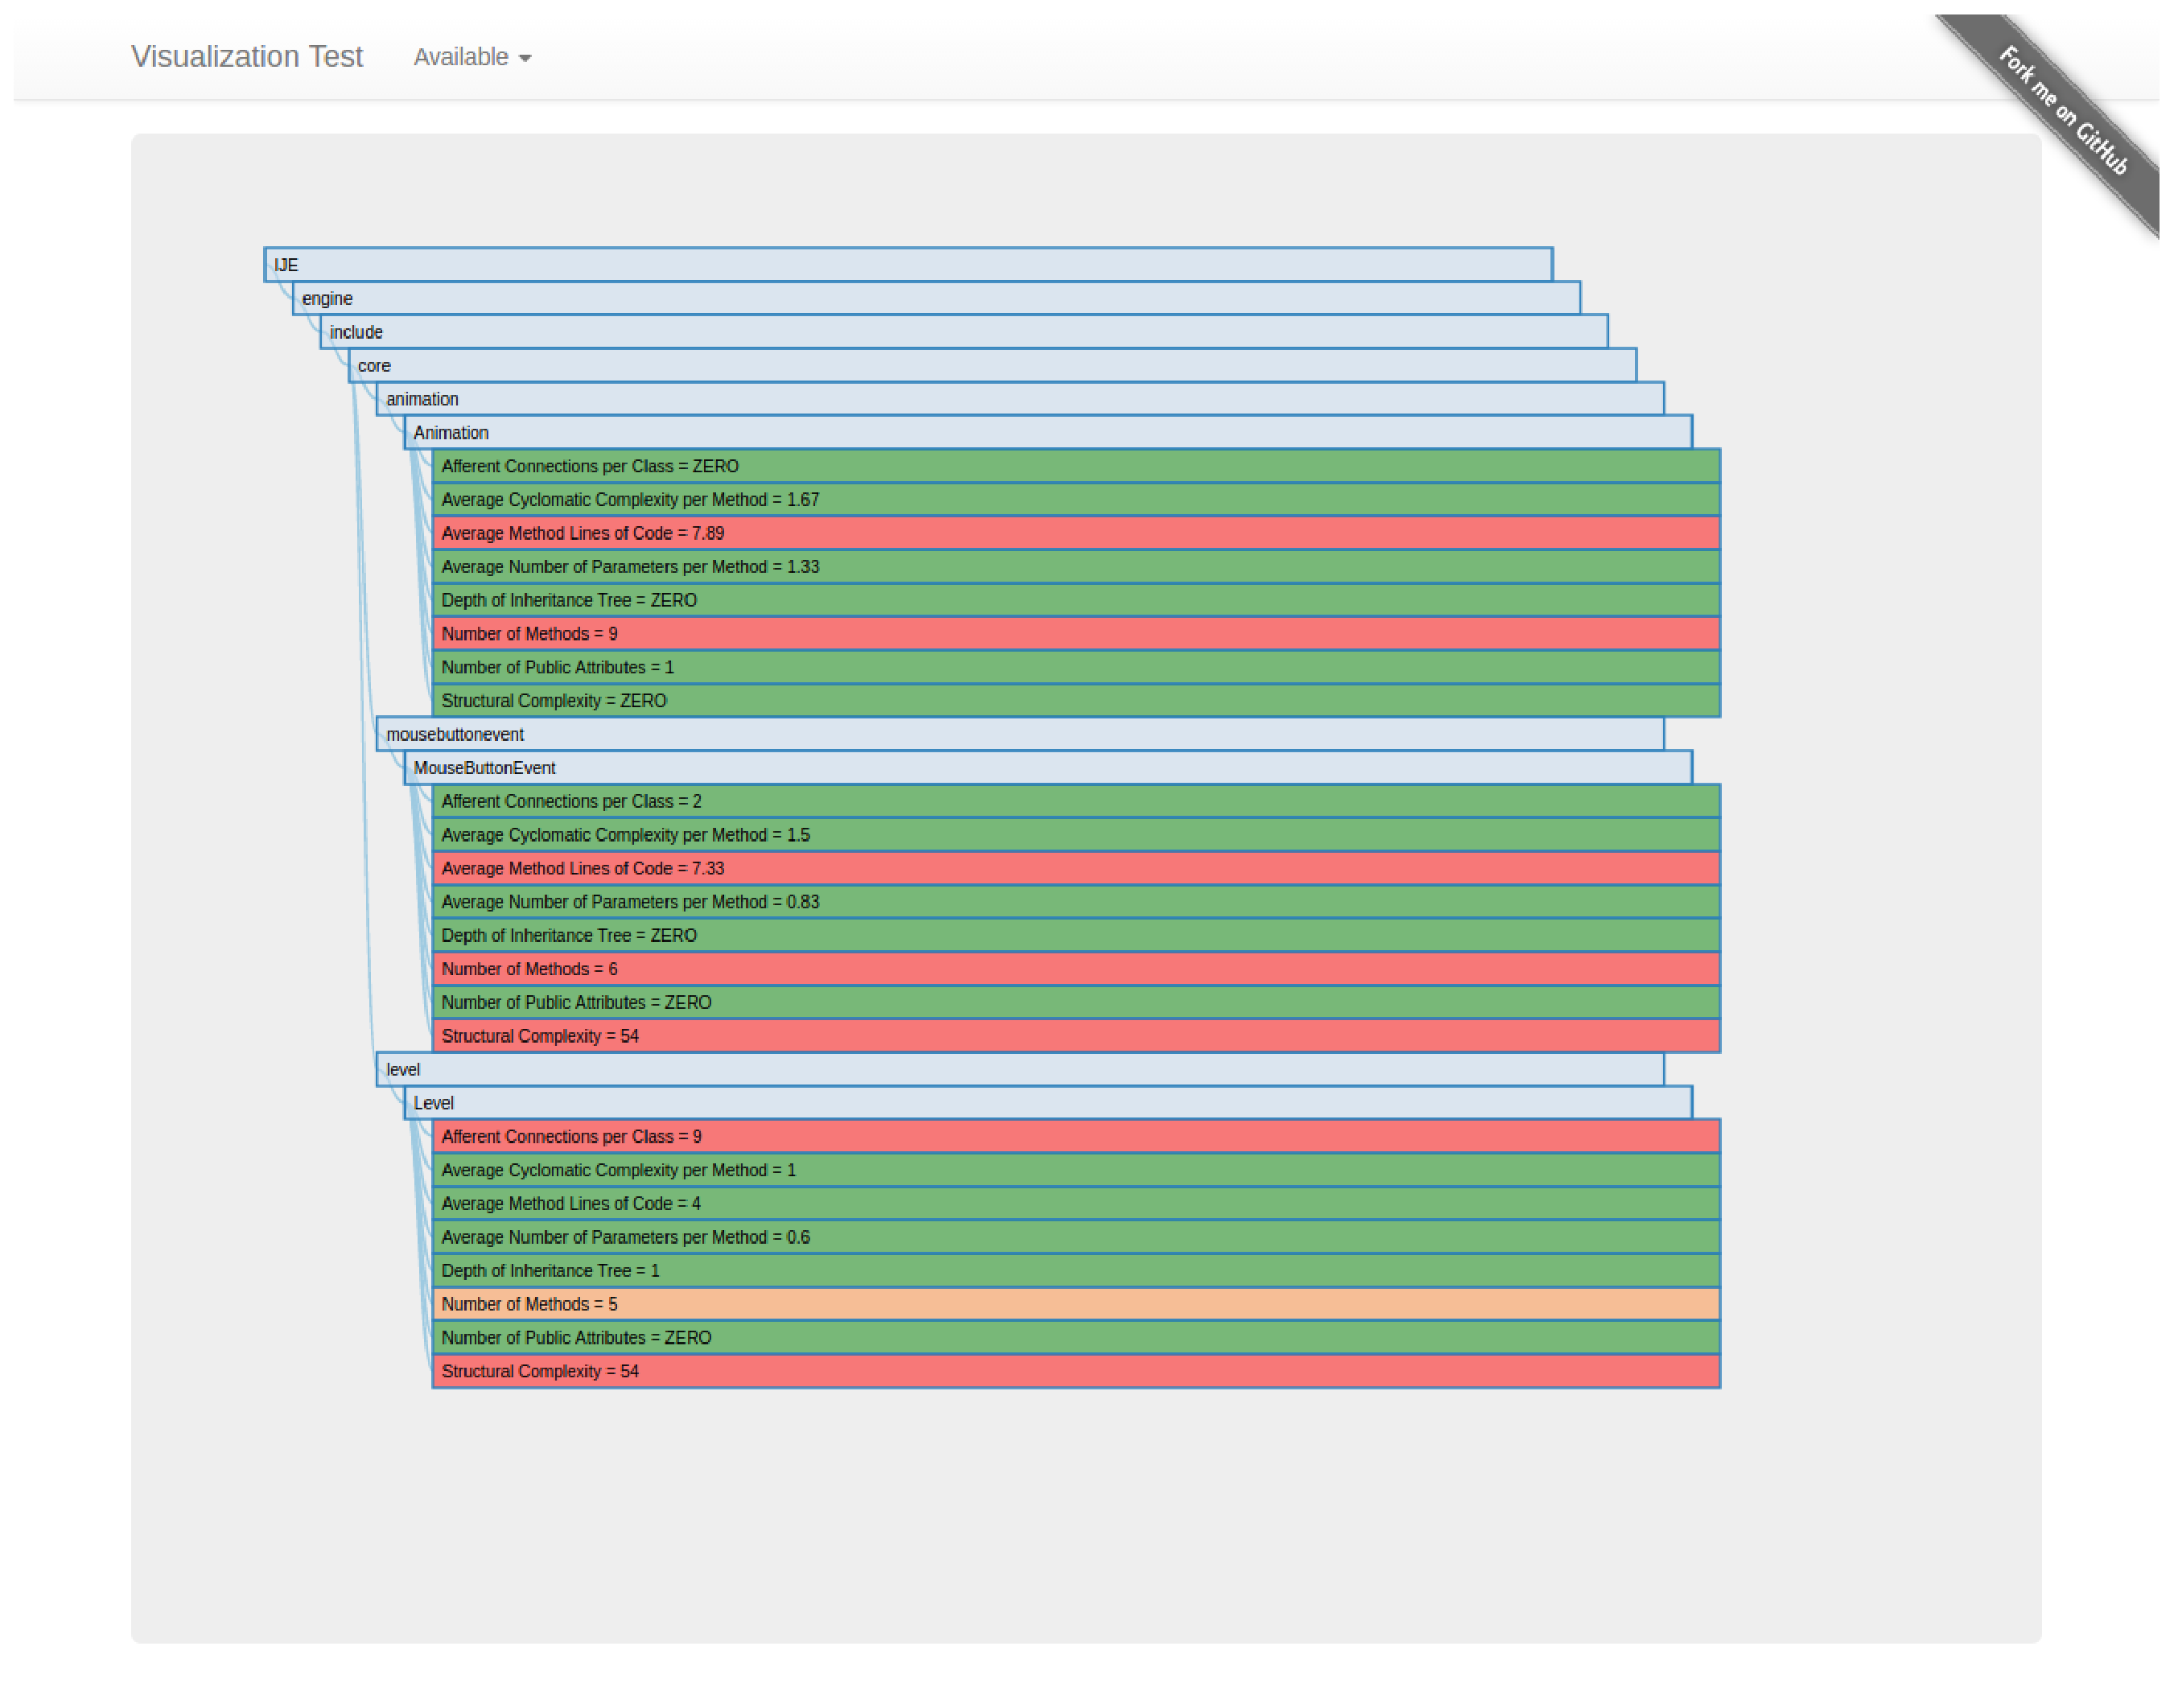
\includegraphics[keepaspectratio=true,scale=0.35]
    {figuras/node_link_tree_with_interaction.eps}
  \caption{Collapsible Indented Tree por Lars Kotthoff (adaptado)}
  \label{fig:node_link_tree_with_interaction}
\end{figure}

\newpage

\newpage

Com um total de 18 participantes, aproximadamente 60\% escolheu a visualização
feita por Lars Kotthoff (Node Link with Interaction - Collapsible Indented
Tree) como a melhor para interpretação das métricas e também para identificar
com mais claridade os pontos críticos. Os resultados completos estão no Anexo
\ref{chap:anexoA}.

\subsection{Resultados Econtrados}

\section{Visualização - Gráfico Radar}
